\documentclass[11pt,a4paper]{article}
\usepackage[T1]{fontenc}
\usepackage[utf8]{inputenc}
\usepackage{mathpazo}
\usepackage[margin=2.3cm]{geometry}
\usepackage{amsmath,amssymb,mathtools}
\usepackage{booktabs,tabularx,array,longtable}
\usepackage{xcolor}
\usepackage{enumitem}
\usepackage{microtype}
\usepackage[most]{tcolorbox}
\usepackage[ruled,vlined,linesnumbered]{algorithm2e}
\usepackage{tikz}
\usetikzlibrary{decorations.pathreplacing,calc,positioning,arrows.meta}
\usepackage[hidelinks]{hyperref}
\usepackage{titlesec}
\usepackage{fancyhdr}

\definecolor{ink}{HTML}{1F2937}
\definecolor{accent}{HTML}{1D4ED8}
\definecolor{soft}{HTML}{EEF2FF}
\definecolor{warn}{HTML}{B45309}
\definecolor{warnsoft}{HTML}{FFF7ED}
\definecolor{drive}{HTML}{3B82F6}
\definecolor{serv}{HTML}{F59E0B}
\definecolor{brk}{HTML}{10B981}
\definecolor{depot}{HTML}{9CA3AF}
\definecolor{wait}{HTML}{E5E7EB}

\titleformat{\section}{\normalfont\Large\bfseries\color{ink}}{\thesection}{0.7em}{}
\titleformat{\subsection}{\normalfont\large\bfseries\color{ink}}{\thesubsection}{0.6em}{}
\setlength{\parskip}{4pt}\setlength{\parindent}{0pt}
\setlist{itemsep=2pt,topsep=2pt}
\renewcommand{\arraystretch}{1.3}
\pagestyle{fancy}\fancyhf{}\renewcommand{\headrulewidth}{0pt}
\fancyfoot[L]{\small\color{gray}legalvrp V0 --- model validation}
\fancyfoot[R]{\small\color{gray}\thepage}

\newcommand{\ok}{$\square$}
\newtcolorbox{words}{colback=soft,colframe=soft,boxrule=0pt,arc=2pt,left=6pt,right=6pt,top=3pt,bottom=3pt}
\newtcolorbox{decide}[1]{colback=warnsoft,colframe=warn,boxrule=0.6pt,arc=2pt,left=6pt,right=6pt,top=4pt,bottom=4pt,
  title={\small\bfseries #1},coltitle=warn,colbacktitle=warnsoft,fonttitle=\bfseries}
\newcommand{\cons}[2]{\par\smallskip\noindent\textbf{\color{accent}#1}\quad #2\par}
\newcommand{\why}[1]{{\small\color{gray!70!black}\emph{Why this form.} #1}\par}

\newcommand{\DB}{\mathrm{DB}}\newcommand{\WB}{\mathrm{WB}}\newcommand{\BR}{\mathrm{BR}}
\newcommand{\DD}{\mathrm{DD}}\newcommand{\DS}{\mathrm{DS}}\newcommand{\WD}{\mathrm{WD}}
\newcommand{\visit}{\mathrm{visit}}\newcommand{\used}{\mathrm{used}}
\newcommand{\drive}{\mathrm{drive}}\newcommand{\brk}{\mathrm{brk}}

\begin{document}

\begin{center}
{\LARGE\bfseries\color{ink} legalvrp V0 --- Model validation}\\[6pt]
{\large Assumptions, variables, constraints and method of the daily MILP}\\[4pt]
{\color{gray} For review and sign-off before implementation}
\end{center}

\vspace{4pt}
\begin{words}
\textbf{How to use this document.} Every assumption (§2) and every constraint (§6) has a box \ok. Tick it if you agree; write a note next to it if not. Anything you change goes back into \texttt{PROJECT\_BRIEF.md} §6 and \texttt{docs/MODEL.md} before code is written. §11 lists the decisions that are genuinely yours to make.
\end{words}

{\small\tableofcontents}

%==================================================================
\section{The problem in five lines}

A regional distributor delivers pallets from one depot with rigid trucks over 3.5\,t. Each afternoon it plans the next day: which driver serves which order, in what sequence, where the legal break is taken, and which orders are postponed. Plans must respect truck capacity, receiving windows, access and equipment, EU driving-time rules, EU and French working-time rules, shifts, and the hours each driver has already worked this week. V0 plans one week, Monday to Friday, as five daily MILPs solved exactly with Gurobi, each passing the drivers' weekly state to the next.

\begin{center}\small
\begin{tabular}{@{}lccc@{}}
\toprule
& \textbf{tiny} & \textbf{small (main)} & \textbf{scale} \\
\midrule
Days & 1 & 5 (Mon--Fri, rolling) & 1 \\
Drivers & 2 & 4 (3 full-time, 1 part-time) & $\lceil n/5\rceil$ \\
Orders per day & 6--8 & 15--20 & $n \in \{8,\dots,40\}$ \\
Purpose & tests, CI & the V0 result & complexity measurement \\
\bottomrule
\end{tabular}
\end{center}

%==================================================================
\section{Assumptions}

Every assumption below is \emph{conservative}: if it is wrong, the model may reject a legal plan, but it never accepts an illegal one --- except where stated.

\begin{center}\small
\begin{longtable}{@{}p{0.7cm}p{6.1cm}p{6.6cm}c@{}}
\toprule
\textbf{\#} & \textbf{Assumption} & \textbf{Why, and what it costs} & \textbf{OK} \\
\midrule
\endhead
\multicolumn{4}{@{}l}{\textit{Scope}}\\
A1 & One depot; every duty starts and ends there the same day & Regional distribution. Excludes long-haul nights out & \ok \\
A2 & One driver drives one fixed truck all week & Avoids driver--truck swaps & \ok \\
A3 & Travel times deterministic, time-independent, integer minutes & No congestion model in V0 & \ok \\
A4 & Service times deterministic ($\sigma = 0$) & ML layer comes later; the field already exists & \ok \\
A5 & Orders of day $d$ are known at $d-1$; no re-planning during the day & Matches the D$-1$ dispatching process & \ok \\
\multicolumn{4}{@{}l}{\textit{Legal interpretation}}\\
A6 & At most \textbf{one} break per duty, 45 min, unsplit & Enough for both break rules because daily driving $\le 9$\,h $= 2\times 4$\,h30 and daily work $\le 12$\,h $= 2\times 6$\,h. Forgoes split breaks & \ok \\
A7 & The break is taken \textbf{at a customer, right after service} & Makes the model linear. Forgoes en-route breaks; harmless while no leg exceeds 4\,h30 & \ok \\
A8 & One break resets both counters (driving and work) & How drivers behave; to confirm against official guidance & \ok \\
A9 & Waiting at a customer counts as \textbf{work}, never as a break & Conservative for the 6\,h rule & \ok \\
A10 & 45 min of break whenever work exceeds 6\,h & The law asks only 30 min between 6 and 9\,h; slight over-protection & \ok \\
A11 & Daily driving cap is 9\,h; the twice-a-week 10\,h extension is disabled & Simplicity; it is a per-driver weekly counter to add later & \ok \\
A12 & Same shift start every day for a given driver & Makes the 11\,h daily rest automatic (on duty $\le 12$\,h45, so off duty $\ge 11$\,h15); still checked & \ok \\
A13 & \emph{Temps de service} = everything on duty except the break: driving, service, waiting, depot prep $P$ and close $R$ & Follows the official definition (driving + other work + waiting) & \ok \\
\multicolumn{4}{@{}l}{\textit{Economics}}\\
A14 & A salaried driver's hours below the contract threshold carry only a tie-breaker cost (0.01\,€/min) & They are already paid; the real levers are km, extra hours, temps and postponements & \ok \\
A15 & Every order may be postponed to the next day at a penalty $p_i$; Friday leftovers are reported unserved & Keeps every day feasible; see §6.8 & \ok \\
A16 & Monetary values are illustrative & Calibrate from CNR indices if you want realism & \ok \\
\bottomrule
\end{longtable}
\end{center}

%==================================================================
\section{One duty, drawn}

The figure fixes the meaning of the time quantities the constraints use. Numbers are illustrative.

\begin{center}
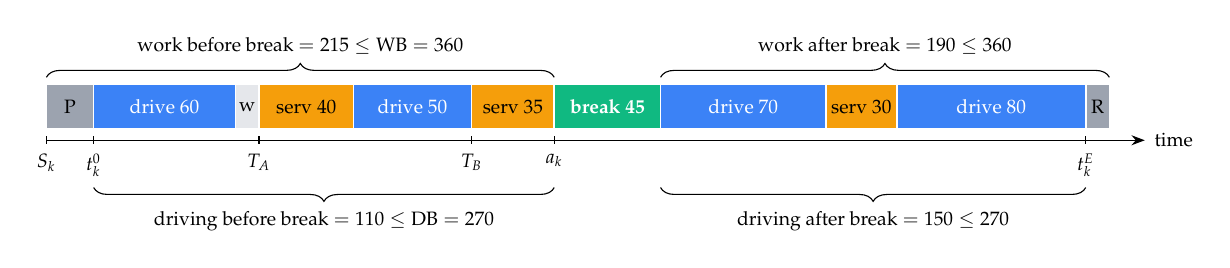
\begin{tikzpicture}[x=0.03cm,y=1cm,font=\scriptsize]
\def\seg#1#2#3#4{\fill[#3] (#1,0) rectangle (#2,0.55); \draw[white,line width=0.6pt] (#1,0) -- (#1,0.55); \node at ({(#1+#2)/2},0.275) {#4};}
\seg{0}{20}{depot}{P}
\seg{20}{80}{drive}{\color{white}drive 60}
\seg{80}{90}{wait}{w}
\seg{90}{130}{serv}{serv 40}
\seg{130}{180}{drive}{\color{white}drive 50}
\seg{180}{215}{serv}{serv 35}
\seg{215}{260}{brk}{\color{white}\textbf{break 45}}
\seg{260}{330}{drive}{\color{white}drive 70}
\seg{330}{360}{serv}{serv 30}
\seg{360}{440}{drive}{\color{white}drive 80}
\seg{440}{450}{depot}{R}
\draw[-{Stealth}] (0,-0.15) -- (465,-0.15) node[right]{time};
\foreach \t/\lab in {0/{$S_k$},20/{$t^0_k$},90/{$T_{A}$},180/{$T_{B}$},215/{$a_k$},440/{$t^E_k$}}{
  \draw (\t,-0.1) -- (\t,-0.2); \node[below] at (\t,-0.2) {\lab};}
\draw[decorate,decoration={brace,amplitude=5pt}] (0,0.65) -- (215,0.65) node[midway,above=5pt]{work before break $=215 \le \WB=360$};
\draw[decorate,decoration={brace,amplitude=5pt}] (260,0.65) -- (450,0.65) node[midway,above=5pt]{work after break $=190 \le 360$};
\draw[decorate,decoration={brace,amplitude=5pt,mirror}] (20,-0.75) -- (215,-0.75) node[midway,below=5pt]{driving before break $=110 \le \DB=270$};
\draw[decorate,decoration={brace,amplitude=5pt,mirror}] (260,-0.75) -- (440,-0.75) node[midway,below=5pt]{driving after break $=150 \le 270$};
\end{tikzpicture}
\end{center}

\begin{words}
\textbf{Definitions used everywhere.} \emph{Driving} = sum of travel times. \emph{Work} = elapsed time on duty excluding the break (waiting included). \emph{Temps de service} $\theta_k$ = from $S_k$ (start of prep) to $t^E_k+R$ (end of close), minus the break: here $450 - 45 = 405$ minutes. The break sits right after a service (A7); the 45 minutes delay the next departure.
\end{words}

%==================================================================
\section{Notation and parameters}

\begin{center}\small
\begin{tabularx}{\textwidth}{@{}l X r@{}}
\toprule
\textbf{Symbol} & \textbf{Meaning} & \textbf{Value / unit} \\
\midrule
$C$ & orders of the day (including those postponed from yesterday) & \\
$0,\ E$ & depot departure node, depot return node & \\
$K$ & drivers working that day & \\
$C_k$ & orders compatible with driver $k$ (truck size vs access, tail-lift, pallets $\le$ capacity) & \\
$A_k$ & arcs of driver $k$: $(0,j)$, $(i,j)$ with $i\ne j$, $(i,E)$, and $(0,E)$ = empty route & \\
$\tau_{ij},\ d_{ij}$ & travel time, distance (asymmetric allowed) & min, km \\
$[e_i, l_i]$ & window for the \emph{start} of service & min from midnight \\
$s_i,\ q_i$ & service duration, pallets & min, pallets \\
$Q_k$ & truck capacity & pallets \\
$S_k,\ F_k$ & shift start, latest end of duty & min \\
$P,\ R$ & depot prep before departure, depot close after return & 20, 10 min \\
$\DB,\ \WB$ & max driving / work between breaks & 270, 360 min \\
$\BR$ & break length & 45 min \\
$\DD,\ \DS$ & max driving / \emph{temps de service} per day & 540, 720 min \\
$\WD$ & max driving per week & 3360 min \\
$W_k,\ V_k$ & service / driving minutes already worked this week (state) & min \\
$H^{\mathrm{thr}}_k,\ H^{\max}_k$ & weekly threshold for extra pay, weekly service cap & e.g.\ 2340, 3120 min \\
$c^{\mathrm{km}}$ & cost per km & 1.60 €/km (illustr.) \\
$c^{\mathrm{reg}}_k,\ c^{\mathrm{ext}}_k$ & cost per regular / extra minute & 0.01, 0.45 €/min (illustr.) \\
$c^{\mathrm{fix}}_k$ & fixed cost if the driver works (temp agency day fee) & € \\
$p_i$ & postponement penalty & 200 €/order (illustr.) \\
\bottomrule
\end{tabularx}
\end{center}

\textbf{Arc pruning (preprocessing).} Arc $(i,j)$ is not created if $e_i + s_i + \tau_{ij} > l_j$: even with no waiting and no break, $j$ would be reached too late. Incompatible (driver, order) pairs create no variables at all.

%==================================================================
\section{Decision variables}

\begin{center}\small
\begin{tabularx}{\textwidth}{@{}l l l X c@{}}
\toprule
\textbf{Code} & \textbf{Symbol} & \textbf{Domain} & \textbf{Meaning} & \textbf{OK}\\
\midrule
\texttt{x[i,j,k]} & $x_{ijk}$ & $\{0,1\}$ & driver $k$ travels arc $(i,j)$ & \ok\\
\texttt{u[i]} & $u_i$ & $\{0,1\}$ & order $i$ is postponed & \ok\\
\texttt{T[i,k]} & $T_{ik}$ & $[e_i, l_i]$ & service start at $i$ (meaningful if $k$ visits $i$) & \ok\\
\texttt{D[i,k]} & $D_{ik}$ & $[0, \DD]$ & driving accumulated on arrival at $i$ & \ok\\
\texttt{y[i,k]} & $y_{ik}$ & $\{0,1\}$ & $k$ takes the break right after serving $i$ & \ok\\
\texttt{t0[k]} & $t^0_k$ & $[S_k+P,\ F_k]$ & departure from the depot & \ok\\
\texttt{tE[k]} & $t^E_k$ & $[S_k+P,\ F_k-R]$ & return to the depot & \ok\\
\texttt{a[k]} & $a_k$ & $[S_k, F_k]$ & start of the break & \ok\\
\texttt{b[k]} & $b_k$ & $[0, \DD]$ & driving accumulated when the break starts & \ok\\
\texttt{svc[k]} & $\theta_k$ & $[0, \DS]$ & \emph{temps de service} today & \ok\\
\texttt{ext[k]} & $o_k$ & $\ge 0$ & weekly minutes above the threshold, after today & \ok\\
\bottomrule
\end{tabularx}
\end{center}

\textbf{Shorthand expressions} (not variables):
$\visit_{ik} = \sum_{j} x_{jik}$ \;(does $k$ serve $i$),\quad
$\used_k = 1 - x_{0Ek}$,\quad
$\drive_k = \sum_{(i,j)} \tau_{ij} x_{ijk}$,\quad
$\brk_k = \sum_i y_{ik}$ \;(0 or 1).

%==================================================================
\section{Objective and constraints}

\subsection{Objective}

\[
\min\ \sum_{k\in K}\Big[\underbrace{c^{\mathrm{km}}\!\!\sum_{(i,j)\in A_k}\!\! d_{ij}x_{ijk}}_{\text{distance}}
+ \underbrace{c^{\mathrm{reg}}_k\,\theta_k}_{\text{tie-breaker}}
+ \underbrace{c^{\mathrm{ext}}_k\,o_k}_{\text{extra hours}}
+ \underbrace{c^{\mathrm{fix}}_k\,\used_k}_{\text{temp day fee}}\Big]
+ \sum_{i\in C}\underbrace{p_i\,u_i}_{\text{postponement}}
\qquad \text{\ok}
\]
\begin{words}
Cost of tomorrow. Because $o_k$ counts the whole week's minutes above the threshold, a driver who was already above it before today contributes a constant; it does not change which plan is optimal. The KPI reports only today's increment.
\end{words}

\subsection{Covering and routing}

\cons{C1 cover \ok}{$\displaystyle\sum_{k:\,i\in C_k}\visit_{ik} + u_i = 1 \qquad \forall i\in C$}
\begin{words}Each order is served by exactly one compatible driver, or postponed.\end{words}

\cons{C2 leave \ok}{$\displaystyle\sum_{j}x_{0jk} = 1 \qquad \forall k$}
\begin{words}Each driver has exactly one route; an idle driver takes the empty arc $(0,E)$.\end{words}

\cons{C3 flow \ok}{$\displaystyle\sum_{j}x_{jik} = \sum_{j}x_{ijk} \qquad \forall k,\ i\in C_k$}
\begin{words}A driver who arrives at a customer leaves it.\end{words}

\cons{C4 capacity \ok}{$\displaystyle\sum_{i}q_i\,\visit_{ik} \le Q_k \qquad \forall k$}
\begin{words}Delivery only, loaded once at the depot: the total load is all that matters.\end{words}

\subsection{Time}

\cons{C5 time from depot \ok}{$T_{jk} \ge t^0_k + \tau_{0j} - M^{0}_{jk}(1-x_{0jk})$}
\cons{C6 time between customers \ok}{$T_{jk} \ge T_{ik} + s_i + \BR\,y_{ik} + \tau_{ij} - M_{ij}(1-x_{ijk})$}
\cons{C7 time back to depot \ok}{$t^E_k \ge T_{ik} + s_i + \BR\,y_{ik} + \tau_{iE} - M^{E}_{ik}(1-x_{iEk})$, \quad and \quad $t^E_k \ge t^0_k$}
\begin{words}If $k$ uses an arc, the next service cannot start before the previous one ends, the break (if taken there) is over, and the travel is done. Waiting is allowed ($\ge$). The windows are the variable bounds of $T_{ik}$.\end{words}
\why{Because every $s_i + \tau_{ij} > 0$, these constraints also forbid subtours (time cannot go round in a circle), so no separate subtour elimination is needed.}

\subsection{Driving accumulation}

\cons{C8 from depot \ok}{$\tau_{0j} - \DD(1-x_{0jk}) \;\le\; D_{jk} \;\le\; \tau_{0j} + \DD(1-x_{0jk})$}
\cons{C9 between customers \ok}{$D_{ik} + \tau_{ij} - (\DD+\tau_{ij})(1-x_{ijk}) \;\le\; D_{jk} \;\le\; D_{ik} + \tau_{ij} + \DD(1-x_{ijk})$}
\begin{words}$D_{jk}$ is \emph{exactly} the driving done before reaching $j$ on $k$'s route.\end{words}
\why{Both sides are needed. With the lower side only, the solver may \emph{inflate} $D$ at the break node, so the driving \emph{after} the break looks shorter than it is. §9 shows a concrete plan that this error accepts illegally. The lower big-M is $\DD+\tau_{ij}$, not $\DD$: otherwise a heavily-driven node could wrongly constrain a successor through an unused arc.}

\subsection{The break}

\cons{C10 where \ok}{$y_{ik} \le \visit_{ik}\quad\forall i$; \qquad $\brk_k \le 1$}
\begin{words}A break only at a customer the driver actually serves; at most one break.\end{words}
\cons{C11 when \ok}{$T_{ik}+s_i - M^{a}_{ik}(1-y_{ik}) \;\le\; a_k \;\le\; T_{ik}+s_i + M^{a}_{ik}(1-y_{ik})$}
\cons{C12 driving at the break \ok}{$D_{ik} - \DD(1-y_{ik}) \le b_k \le D_{ik} + \DD(1-y_{ik})$; \qquad $b_k \le \DD\,\brk_k$}
\begin{words}If the break is after $i$, then $a_k$ is the end of service at $i$ and $b_k$ is the driving done so far. Without a break, $b_k = 0$.\end{words}

\subsection{Legal limits within the day}

\cons{C13 driving segments \ok}{$b_k \le \DB$; \qquad $\drive_k - b_k \le \DB$}
\begin{words}At most 4\,h30 of driving before the break and after it. With no break ($b_k=0$) this reads: total driving $\le$ 4\,h30.\end{words}

\cons{C14 work segments \ok}{
$\begin{aligned}[t]
a_k - (t^0_k - P) &\le \WB + M^{w}_k(1-\brk_k) && \text{work before the break}\\
(t^E_k + R) - (a_k + \BR) &\le \WB + M^{w}_k(1-\brk_k) && \text{work after the break}\\
(t^E_k + R) - (t^0_k - P) &\le \WB + M^{w}_k\,\brk_k && \text{no break: whole duty}
\end{aligned}$}
\begin{words}At most 6\,h of work without a break. Prep $P$ is work before the first segment; close $R$ is work at the end of the last one.\end{words}
\why{Leaving $R$ out accepts plans that are illegal by up to 10 minutes. It was spotted by derivation while preparing the tests; the brute-force comparison of §9 then confirms it is detectable (1 instance in 15).}

\cons{C15 daily driving \ok}{$\drive_k \le \DD$}

\subsection{Service time and the week}

\cons{C16 service time \ok}{$\theta_k \ge (t^E_k + R) - (t^0_k - P) - \BR\,\brk_k - M^{w}_k(1-\used_k)$, \qquad $\theta_k \le \DS$}
\begin{words}Today's \emph{temps de service}, capped at 12\,h. An idle driver has $\theta_k = 0$, so idle days do not consume weekly hours.\end{words}
\why{$\theta_k$ is bounded from below only; it can be over-estimated but never under-estimated, which is the safe direction for every cap. Reported values and the next day's state are recomputed from the routes, never read from $\theta_k$.}

\cons{C17 weekly caps \ok}{$W_k + \theta_k \le H^{\max}_k$; \qquad $V_k + \drive_k \le \WD$}
\cons{C18 extra minutes \ok}{$o_k \ge W_k + \theta_k - H^{\mathrm{thr}}_k$, \qquad $o_k \ge 0$}
\begin{words}The week enters the day here: the same route is cheaper for a driver at 20\,h than for one at 37\,h.\end{words}

\subsection{Optional: identical drivers}

If drivers $k$ and $k+1$ are identical (contract, truck, shift, state), add $\sum_i\visit_{ik} \ge \sum_i\visit_{i,k+1}$ to remove mirror solutions. \ok

\subsection{A property worth knowing}

\begin{words}
\textbf{Every day is feasible by construction.} Postponing all orders and leaving all drivers idle satisfies every constraint, provided yesterday's plan was legal ($W_k \le H^{\max}_k$) and $P + R \le \WB$. So an \texttt{INFEASIBLE} status can only mean inconsistent input data.
\end{words}

%==================================================================
\section{Which rule is enforced where}

\begin{center}\small
\begin{tabularx}{\textwidth}{@{}X l l@{}}
\toprule
\textbf{Rule} & \textbf{Source} & \textbf{Constraints} \\
\midrule
45 min break after at most 4\,h30 of driving & Reg.\ (EC) 561/2006 art.\ 7 & C10--C13 \\
No more than 6\,h of work without a break & Dir.\ 2002/15/EC art.\ 5; C.\ transports L3312-2 & C10--C12, C14 \\
Break $\ge$ 30 / 45 min if work 6--9\,h / $>$9\,h & same & C14 with A10 \\
Daily driving $\le$ 9\,h & 561/2006 art.\ 6 & C15 \\
Daily \emph{temps de service} $\le$ 12\,h & C.\ transports D3312-51 & C16 \\
Weekly driving $\le$ 56\,h & 561/2006 art.\ 6 & C17 \\
Weekly \emph{temps de service} $\le$ 52\,h, extra pay above threshold & C.\ transports D3312-45, -50 & C17, C18 \\
Daily rest $\ge$ 11\,h & 561/2006 art.\ 8 & A12 + week-loop check \\
Receiving windows & commercial & bounds of $T$, C5--C7 \\
Capacity, access, tail-lift & physical & C4, sets $C_k$ \\
Shift start and latest end & roster & bounds of $t^0$, $t^E$ \\
\bottomrule
\end{tabularx}
\end{center}

%==================================================================
\section{Big-M values}

Each big-M is the smallest value that switches its constraint off when the controlling binary is 0. Never use one global constant: loose big-M values are the main cause of slow MILPs of this type.

\begin{center}\small
\begin{tabularx}{\textwidth}{@{}l l X@{}}
\toprule
\textbf{Where} & \textbf{Value} & \textbf{Reasoning} \\
\midrule
C5 & $M^0_{jk} = \max(0,\ F_k + \tau_{0j} - e_j)$ & latest departure $+$ travel, minus earliest possible $T_j$ \\
C6 & $M_{ij} = \max(0,\ l_i + s_i + \BR + \tau_{ij} - e_j)$ & latest end at $i$ incl.\ break, minus earliest $T_j$ \\
C7 & $M^E_{ik} = \max(0,\ l_i + s_i + \BR + \tau_{iE} - S_k - P)$ & same, against the earliest return \\
C11 & $M^a_{ik} = \max(F_k, l_i+s_i) - \min(S_k, e_i+s_i)$ & full range of $a_k - (T_{ik}+s_i)$ \\
C14, C16 & $M^w_k = F_k - S_k + P + R$ & longest possible duty \\
C8, C12, upper C9 & $\DD$ & range of accumulated driving \\
lower C9 & $\DD + \tau_{ij}$ & $D_{ik}$ can reach $\DD$ on an unused arc \\
\bottomrule
\end{tabularx}
\end{center}

%==================================================================
\section{Evidence that the model is right}

Before writing the brief, the formulation was implemented in a scratch script and compared against \emph{exhaustive enumeration} (every assignment, sequence, postponement, break position and integer departure minute) on small days with 5 orders and 2 drivers, in three regimes.

\begin{center}\small
\begin{tabular}{@{}lccc@{}}
\toprule
\textbf{Model variant} & \textbf{mixed (12)} & \textbf{work-heavy (15)} & \textbf{driving-heavy (15)} \\
\midrule
\textbf{Formulation of this document} & \textbf{0 mismatches} & \textbf{0} & \textbf{0} \\
Break delay removed from C6--C7 & --- & 15 / 15 detected & --- \\
C14 without $R$ & 0 / 12 & 1 / 15 detected & --- \\
C9 lower side only & --- & 0 / 15 & 0 / 15 \\
C9 lower big-M $= \DD$ & 0 / 12 & 0 / 15 & 0 / 15 \\
\bottomrule
\end{tabular}
\end{center}

Random instances do not catch every error. The one-sided C9 is only exposed by a handcrafted case --- the \textbf{trap}, which becomes a mandatory test:

Route depot $\to$ A $\to$ B $\to$ C $\to$ depot, legs of 60, 140, 200 and 140 minutes; driving on arrival is 60 at A, 200 at B, 400 at C, and 540 in total.

\begin{center}\small
\begin{tabular}{@{}lccc@{}}
\toprule
\textbf{Break after} & \textbf{Driving before} & \textbf{Driving after} & \textbf{4\,h30 rule} \\
\midrule
A & 60 & 480 & violated \\
B & 200 & 340 & violated \\
C & 400 & 140 & violated \\
none & --- & 540 & violated \\
\bottomrule
\end{tabular}
\end{center}

No break position makes this route legal. The correct model postpones one order (cost 1\,532.40\,€); the model with a one-sided C9 serves all three illegally (cost 742.00\,€).

The lower big-M of C9 was not caught by any test either; it is corrected by derivation (§8), not by evidence.

%==================================================================
\section{Method}

\subsection{One day}

\begin{enumerate}[label=\arabic*.]
\item \textbf{Prepare.} Compatibility sets $C_k$; arc pruning; big-M values.
\item \textbf{Baseline (status quo).} k-means territories, one per driver; Hungarian assignment of territories to drivers; nearest neighbour then 2-opt; the route evaluator chooses the break position and the departure time. Orders that fit nowhere are postponed.
\item \textbf{Solve.} Build the MILP of §6, give the baseline as a MIP start, solve with Gurobi (120\,s, 1\,\% gap for \emph{small}).
\item \textbf{Extract} routes, break positions and times.
\item \textbf{Check.} The independent checker recomputes every time from the plan and verifies every rule. Zero violations is mandatory.
\item \textbf{Fallback.} No incumbent at the time limit $\Rightarrow$ keep the baseline plan and flag the day.
\end{enumerate}

\subsection{The week}

\begin{algorithm}[h]
\caption{Rolling week (Monday to Friday)}
$W_k \leftarrow 0,\ V_k \leftarrow 0$ for every driver; carry $\leftarrow \emptyset$\;
\For{$d = $ Monday \KwTo Friday}{
  $C \leftarrow$ orders of day $d$ $\cup$ carry \tcp*{carried orders keep their window and penalty}
  plan$_d \leftarrow$ \textsc{SolveDay}($C$, drivers, $W$, $V$) \tcp*{steps 1--6 above}
  \textbf{assert} checker(plan$_d$) $= \emptyset$\;
  \ForEach{driver $k$}{
    $W_k \mathrel{+}= \theta_k$,\ $V_k \mathrel{+}= \drive_k$ \tcp*{recomputed from the route}
    check rest: start$_{d+1} \ge$ end$_d + 11$\,h\;
  }
  carry $\leftarrow$ postponed orders of plan$_d$\;
}
report carry as unserved; compute weekly KPIs; run the week-mode checker\;
\end{algorithm}

\textbf{Known limitation.} The loop is \emph{myopic}: Monday's plan does not know Friday's volume, so it may use a driver's hours early and pay extra time later. Optional task T11 measures this \emph{price of myopia} with a clairvoyant weekly MILP on small instances.

%==================================================================
\section{Size and complexity}

\begin{center}\small
\begin{tabular}{@{}rrrrrc@{}}
\toprule
\textbf{Orders} & \textbf{Drivers} & \textbf{Variables} & \textbf{Constraints} & \textbf{Possible plans} & \textbf{Free pip licence} \\
\midrule
8 & 2 & 214 & 534 & $4\times10^{5}$ & yes \\
13 & 3 & 697 & 1\,852 & $6\times10^{11}$ & yes (limit) \\
20 & 4 & 1\,968 & 5\,440 & $4\times10^{21}$ & no \\
30 & 6 & 6\,192 & 17\,580 & $8\times10^{37}$ & no \\
40 & 8 & 14\,176 & 40\,800 & $5\times10^{55}$ & no \\
\bottomrule
\end{tabular}
\end{center}

Sizes grow as drivers $\times$ orders$^2$ (before arc pruning). Expected behaviour with a 2--5 minute limit: optimal up to about 15 orders a day, small gaps up to about 25, the wrong tool beyond about 40. Task T9 replaces these expectations with measurements.

%==================================================================
\section{Decisions that are yours}

\begin{decide}{D1 --- Break model}
Keep one 45-minute break at a customer (A6, A7)? Alternative: allow the 15\,+\,30 split, i.e.\ two break slots. Doubles the break variables; closer to the law; rarely changes the plan in regional distribution.
\end{decide}

\begin{decide}{D2 --- Waiting counts as work (A9)}
Conservative. Alternative: let waiting of known duration count as availability rather than work, which relaxes the 6\,h rule.
\end{decide}

\begin{decide}{D3 --- Cost of regular hours (A14)}
Tie-breaker only. Alternative: a full hourly cost, which turns the objective into ``minimise hours'' and favours shorter days even when nothing is saved.
\end{decide}

\begin{decide}{D4 --- Postponement penalty}
Fixed 200\,€ per order, constant over the week. Alternative: escalate it for carried orders so a postponed order is not postponed twice.
\end{decide}

\begin{decide}{D5 --- Part-time ceiling}
Contract hours $+$ 10\,\% (Code du travail default). Alternative: up to one third, if a collective agreement allows it.
\end{decide}

\begin{decide}{D6 --- Rolling or clairvoyant as the headline}
Rolling is realistic; clairvoyant is a bound. V0 reports rolling and, optionally, the gap to clairvoyant.
\end{decide}

\vspace{6pt}
\begin{words}
\textbf{Sign-off.} \quad Assumptions A1--A16 \ok \qquad Variables \ok \qquad Constraints C1--C18 \ok \qquad Decisions D1--D6 recorded \ok
\end{words}

\end{document}
